% Original source Fig.31.5, PDF138 / printed126: triangle and three mixed bubbles.
% Fixed labeled external legs: S_triangle=1, S_each_mixed_bubble=2.
% All external momenta incoming. No internal arrow/routing invented for this figure.
% The upper node of each mixed bubble is cubic, the lower node quartic.
% Products below panels identify the factors; they do not include propagators.
% Basic TikZ only; no caption or automatic numbering.
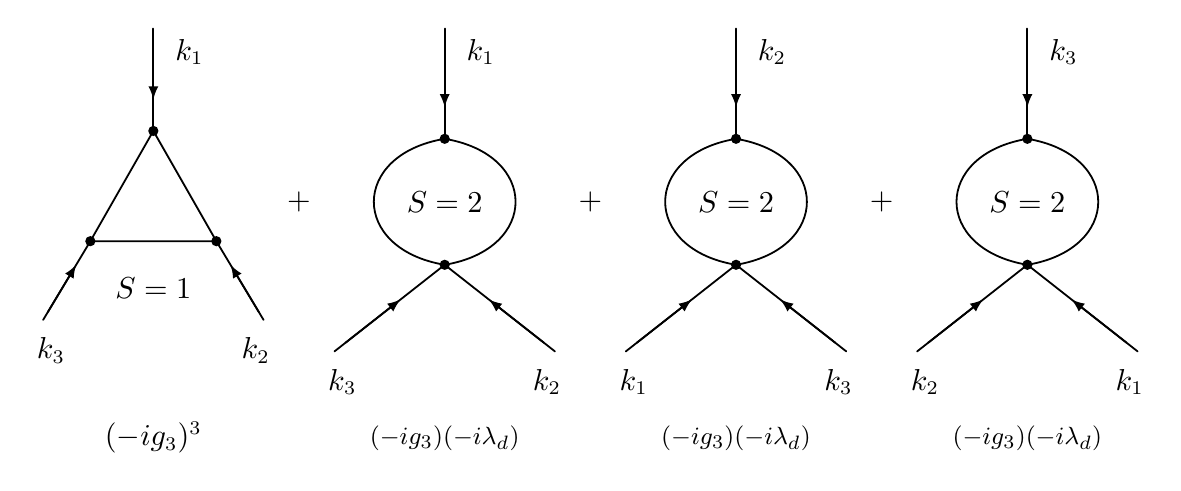
\begin{tikzpicture}[x=1mm,y=1mm,line width=.65pt,>=latex,
  line cap=round,line join=round,
  font=\fontsize{10.5}{12}\selectfont]
\begin{scope}[shift={(17,0)}]
  \draw (0,9) -- (-8,-5) -- (8,-5) -- cycle;
  \draw (0,22) -- (0,9);
  \draw (-14,-15) -- (-8,-5);
  \draw (14,-15) -- (8,-5);
  \draw[->] (0,20) -- (0,13);
  \draw[->] (-13.4,-14) -- (-9.8,-8);
  \draw[->] (13.4,-14) -- (9.8,-8);
  \fill (0,9) circle[radius=.65mm];
  \fill (-8,-5) circle[radius=.65mm];
  \fill (8,-5) circle[radius=.65mm];
  \node[right] at (1.5,19) {$k_1$};
  \node[below] at (-13,-16) {$k_3$};
  \node[below] at (13,-16) {$k_2$};
  \node at (0,-11) {$S=1$};
  \node at (0,-30) {$(-ig_3)^3$};
\end{scope}
\node at (35.5,0) {$+$};
\begin{scope}[shift={(54,0)}]
  \draw (0,8) .. controls (-12,6) and (-12,-6) .. (0,-8);
  \draw (0,8) .. controls (12,6) and (12,-6) .. (0,-8);
  \draw (0,22) -- (0,8);
  \draw (-14,-19) -- (0,-8);
  \draw (14,-19) -- (0,-8);
  \draw[->] (0,20) -- (0,12);
  \draw[->] (-12.6,-17.9) -- (-5.6,-12.4);
  \draw[->] (12.6,-17.9) -- (5.6,-12.4);
  \fill (0,8) circle[radius=.65mm];
  \fill (0,-8) circle[radius=.65mm];
  \node[right] at (1.5,19) {$k_1$};
  \node[below] at (-13,-20) {$k_3$};
  \node[below] at (13,-20) {$k_2$};
  \node at (0,0) {$S=2$};
  \node[font=\fontsize{9.5}{11}\selectfont] at (0,-30) {$(-ig_3)(-i\lambda_d)$};
\end{scope}
\node at (72.5,0) {$+$};
\begin{scope}[shift={(91,0)}]
  \draw (0,8) .. controls (-12,6) and (-12,-6) .. (0,-8);
  \draw (0,8) .. controls (12,6) and (12,-6) .. (0,-8);
  \draw (0,22) -- (0,8);
  \draw (-14,-19) -- (0,-8);
  \draw (14,-19) -- (0,-8);
  \draw[->] (0,20) -- (0,12);
  \draw[->] (-12.6,-17.9) -- (-5.6,-12.4);
  \draw[->] (12.6,-17.9) -- (5.6,-12.4);
  \fill (0,8) circle[radius=.65mm];
  \fill (0,-8) circle[radius=.65mm];
  \node[right] at (1.5,19) {$k_2$};
  \node[below] at (-13,-20) {$k_1$};
  \node[below] at (13,-20) {$k_3$};
  \node at (0,0) {$S=2$};
  \node[font=\fontsize{9.5}{11}\selectfont] at (0,-30) {$(-ig_3)(-i\lambda_d)$};
\end{scope}
\node at (109.5,0) {$+$};
\begin{scope}[shift={(128,0)}]
  \draw (0,8) .. controls (-12,6) and (-12,-6) .. (0,-8);
  \draw (0,8) .. controls (12,6) and (12,-6) .. (0,-8);
  \draw (0,22) -- (0,8);
  \draw (-14,-19) -- (0,-8);
  \draw (14,-19) -- (0,-8);
  \draw[->] (0,20) -- (0,12);
  \draw[->] (-12.6,-17.9) -- (-5.6,-12.4);
  \draw[->] (12.6,-17.9) -- (5.6,-12.4);
  \fill (0,8) circle[radius=.65mm];
  \fill (0,-8) circle[radius=.65mm];
  \node[right] at (1.5,19) {$k_3$};
  \node[below] at (-13,-20) {$k_2$};
  \node[below] at (13,-20) {$k_1$};
  \node at (0,0) {$S=2$};
  \node[font=\fontsize{9.5}{11}\selectfont] at (0,-30) {$(-ig_3)(-i\lambda_d)$};
\end{scope}
\end{tikzpicture}
